\documentclass[../main.tex]{subfiles}
\begin{document}
\chapter{Floating Point Arithmetic and Error Analysis }
\addcontentsline{toc}{section}{Chapter 5:Floating Point Arithmetic and Error Analysis}

\section{FLOATING POINT NUMBERS }

We have already mentioned that the data contained in just a single irrational real number such as $\pi$ has more information in its digits than all the computers in the world could possibly ever store. Then again, it would probably take all the scientific surveyors in the world to look for and not be able to find any scientist who vitally needed, say, the 534th digit of this number. What is usually required in scientific work is to maintain accuracy with a certain number of so-called \textbf{significant digits}, which constitutes the portion of a numerical answer to a problem that is trusted to be correct. For example, if we want $\pi$ to three significant digits, we could use 3.14. A computer can only work with a finite set of numbers; these computer numbers for a given system are usually called floating point numbers. Since there are infinitely many real numbers, what has to happen is that big (infinite) sets of real numbers must get identified with single computer numbers. Floating point numbers are best understood by their relations with numbers in scientific notation, such as $3.14159 \times 10^{0}$, although they need not be written in this form.\\

\textbf{A floating point number system} is determined by a \textbf{base} $\beta$ (any positive integer greater than one), a precision $s$ (any positive integer; this will be the number of significant digits), and two integers $m$ (negative) and $M$ (positive), that determine the exponent range. In such a system, a floating point number can always be expressed in the form:
$$
\pm . d_{1} d_{2} \cdots d_{s} \times \beta^{e},
$$
where,
$$
d_{i}=0,1,2, \cdots, \text { or } \beta-1 \text { but } d_{1} \neq 0 \text { and } m \leq e \leq M .
$$

The number zero is represented as $.00 \cdots 0 \times \beta^{-m}$. In a computer, each of the three parts (the sign $\pm$, mantissa $d_{1} d_{2} \cdots d_{s}$, and the exponent $\beta$ ) of a floating point number is stored in its own separate fixed-width field. Most contemporary computers and software on the market today (MATLAB included) use \textbf{binary arithmetic} $(\beta=2)$. Hand-held calculators use decimal base $\beta=10$. In the past, other computers have used different bases that were usually powers of two, such as $\beta=16$ (hexadecimal arithmetic). Of course, such arithmetic (different from base 10) is done in internal calculations only. When the number is displayed, it is converted to decimal form. An important quantity for determining the precision of a given computing system is known as the \textbf{unit roundoff} $u$ (or the \textbf{umachine epsilon} \footnote{The rationale for this terminology is that the Greek letter epsilon $(\varepsilon)$ is usually used in mathematical analysis to represent a very small number.
}), which is the maximum relative error that can occur when a real number is approximated by a floating point number.\footnote{There is another characterization of the unit roundoff as the gap between the floating point number 1 and the next floating point number to the right. These two definitions are close, but not quite equivalent; see Example 5.4 and Exercise for the Reader 5.3 for more details on how these two quantities are related, as well as explicit formulas for the unit roundoff.}For example, one Texas Instruments graphing calculator uses the floating point parameters $\beta=10, s=12, m=-99$, and $M=99$, which means that this calculator can effectively handle numbers whose absolute values lie (approximately) between $10^{-99}$ and $10^{99}$, and the unit roundoff is $u=10^{-12}$. MATLAB's arithmetic uses the parameters: $\beta=2, s=$ $53, m=-1074$, and $M=1023$, which conforms to the \textbf{IEEE double precision standard}.\footnote{The IEEE (I-triple-E) is a nonprofit, technical professional association of more than 350,000 individual members in 150 countries. The full name is the Institute of Electrical and Electronics Engineers, Inc. The IEEE single-precision (SP) and double-precision (DP) standards have become the intemational standard for computers and numerical software. The standards were carefully developed to help avoid some problems and incompatibilities with previous floating point systems. In our notation, the IEEE SP standard specifies $\beta=2, s=24, m=-126,=-126$, and $M=127$ and the IEEE DP standard has $\beta=2, s=53, m=-1022$, and $M=1023$.} This means that MATLAB can effectively handle numbers with absolute values from $2^{-1074} \approx 10^{-324}$ to $2^{1023} \approx 10^{308}$; also the unit roundoff is $u=$ $2^{-53} \approx 10^{-16}$.

\section{ FLOATING POINT ARITHMETIC: THE BASICS}

Many students have gotten accustomed to the reliability and logical precision of exact mathematical arithmetic. When we get the computer to perform calculations for us, we must be aware that floating point arithmetic compounded with roundoff errors can lead to unexpected and undesirable results. Most large-scale numerical algorithms are not exact algorithms, and when such methods are used, attention must be paid to the error estimates. We saw this at a basic level in Chapter 2, and it will reappear again later on several occasions. Here we will talk about different sorts of errors, namely, those that arise and are compounded by the computer's floating point arithmetic. We stress the distinction with the first type of errors. Even if an algorithm is mathematically guaranteed to work, floating point errors may arise and spoil its success. All of our illustrations below will be in base 10 floating point arithmetic, since all of the concepts can be covered and better understood in this familiar setting; changing to a different base is merely a technical issue. To get a feel for the structure of a floating point number system, we begin with an example of a very small system.

EXAMPLE 5.1: Find all floating point numbers in the system with $\beta=10, s=$ $1, m=-1$, and $M=1$.

SOLUTION: In this case, it is a simple matter to write down all of the floating point numbers in the system:
$$
\begin{array}{ccc}
\pm .1 \times 10^{-1}=\pm .01 & \pm .1 \times 10^{0}=\pm .1 & \pm .1 \times 10^{1}=\pm 1 \\
\pm .2 \times 10^{-1}=\pm .02 & \pm .2 \times 10^{0}=\pm .2 & \pm .2 \times 10^{1}=\pm 2 \\
\vdots & \vdots & \vdots \\
\pm .9 \times 10^{-1}=\pm .09 & \pm .9 \times 10^{0}=\pm .9 & \pm .9 \times 10^{1}=\pm 9 .
\end{array}
$$


\begin{minipage}[t]{.6\linewidth}
Apart from these, there is only $0=.0 \times 10^{-1}$. Of these 55 numbers, the nonnegative ones are pictured on the number line in Figure 5.1. We stress that the gaps between adjacent floating point numbers are not always the same; in general, these gaps become smaller near zero and more spread out far away from zero (larger numbers).

\end{minipage}
\hspace{0.02\linewidth}
\begin{minipage}[t]{.5\linewidth}
  \strut\vspace*{-\baselineskip}\newline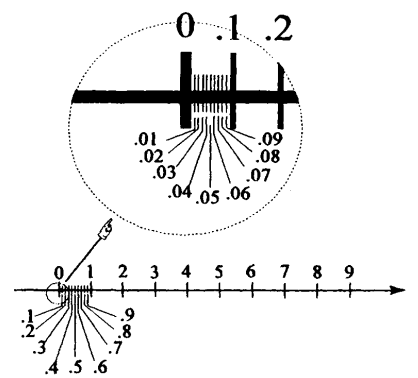
\includegraphics[width=\linewidth]{fig51}
  \captionof{figure}{The nonnegative floating point numbers of Example 5.1. The omitted negative floating point numbers are
just (in any floating point number system) the opposites of the positive numbers shown.
The situation is typical in that as we approach zero, the density of floating point numbers
increases.}
\label{fig:fig_5_1}
\end{minipage}


Let us now talk about how real numbers get converted to floating point numbers. Any real number $x$ can be expressed in the form
$$
x=\pm d_{1} d_{2} \cdots d_{s} d_{s+1} \cdots \times 10^{e}
$$

where there are infinitely many digits (this is the only difference from the floating point representation (1) with $\beta=10$ ) and there is no restriction on the exponent's range. The part $d_{1} d_{2} \cdots d_{s} d_{s+1} \cdots$ is called the mantissa of $x$. If $x$ has a finite decimal expansion, we can trail it with an infinite string of zeros to conform with (2). In fact, the representation (2) is unique for any real number (i.e., there is only one way to represent any $x$ in this way) provided that we adopt the convention that an infinite string of 9 's not be allowed; such expansions should just be rounded up. (For example, the real number .37999999999... is the same as .38.) At first glance, it may seem straightforward how to represent a real number $x$ in form (2) by a floating point number of form (1) with $\beta=10$; simply either chop off or round off any of the digits past the allowed number. But there are serious problems that may arise, stemming from the fact that the exponent $e$ of the real number may be outside the permitted range. Firstly, if $e>M$, this means that $x$ is (probably much) larger than any floating point number and so cannot be represented by one. If such a number were to come up in a computation, the computation is said to have overflowed. For example, in the simple setting of Example 5.1, any number $x \geq 10$ would overflow this simple floating point system. Depending on the computer system, overflows will usually result in termination of calculation or a warning. For example, most graphing calculators, when asked to evaluate an expression like $e^{5000}$, will either produce an error message like "OVERFLOW", and freeze up or perhaps give $\infty$ as an output. MATLAB behaves similarly to the latter pattern for overflows:


\begin{verbatim}
>>exp(5000)
->ans = Inf %MATLAB's abbreviation for infinity.
\end{verbatim}

Inf (or inf) is MATLAB's way of saying the number is too large to continue to do any more number crunching, except for calculations where the answer will be either Inf or - Inf (a very large negative number). Here are some examples:

\begin{verbatim}
>> exp(5000)
->ans = Inf % MATLAB tells us we have a very big positive number here
>> 2*exp(5000)
->ans = Inf %No new information
>> exp(5000)/-5
->ans = -Inf %OK now we have a very big negative number.
>>2*exp(5000)-exp(5000)
->ans = NaN % "NaN" stands for "not a number" 
\end{verbatim}

The last calculation is more interesting. Obviously, the expression being evaluated is just $e^{5000}$, which, when evaluated separately, is outputted as Inf. What happens is that MATLAB tries instead to do inf-inf, which is undefined (once large numbers are converted to inf, their relative sizes are lost and it is no longer possible for MATLAB to compare them).\footnote{We mention that the optional "Symbolic Toolbox" for MATLAB allows, among other things, the symbolic manipulation of such expressions. The Symbolic Toolbox does come with the student version of MATLAB. Some of its features are explained in Appendix A. }

A very different situation occurs if the exponent $e$ of the real number $x$ in (2) is less than $m$ (too small). This means that the real number $x$ has absolute value (usually much) smaller than that of any nonzero floating point number. In this case, a computation is said to have underflowed. Most systems will represent an underflow by zero without any warning, and this is what MATLAB does.

Underflows, although less serious than overflows, can be a great source of problems in large-scale numerical calculations. Here is a simple example. We know from basic rules of exponents that $e^{p} e^{-p}=e^{p-p}=e^{0}=1$, but consider the following calculation:

\begin{verbatim}
>> exp(-5000)
->ans = 0 %this very small number has underflowed to zero
>> exp(5000)*exp(-5000)
->ans = NaN 

\end{verbatim}

The latter calculation had both underflows and overflows and resulted in $0 \star \operatorname{Inf}$ $(=0 \cdot \infty)$, which is undefined. We will give another example shortly of some of the tragedies that can occur as the result of underflows. But now we show two simple ways to convert a real number to a floating point number in case there is no overflow or underflow. So we assume the real number $x$ in (2) has exponent $e$ satisfying $m \leq e \leq M$. The two methods for converting the real number $x$ to its floating point representative $\mathrm{fl}(x)$ are as follows:

\underline{(i) Chopped (or Truncated) Arithmetic}: With this system we simply drop all digits after $d_{s}$ :
$$
\mathrm{fl}(x)=\mathrm{fl}\left(\pm . d_{1} d_{2} \cdots d_{s} d_{s+1} \cdots \times 10^{e}\right)=\pm d_{1} d_{2} \cdots d_{s} \times 10^{e}
$$
\underline{(ii) Rounded Arithmetic}: Here we do the usual rounding scheme for the first $s$ significant digits. If $d_{s+1}<5$, we simply chop as in method (i), but if $d_{s+1} \geq 5$, we need to round up. This may change several digits depending on if there is a string of 9 's or not. For example, with $s=4, \ldots 2456823 \ldots$ would round to $.2457$ (onedigit changed), but $.2999823$ would round to $.3000$ (four digits changed). So a nice formula as in (i) is not possible. There is, however, an elegant way to describe rounded arithmetic in terms of chopped arithmetic using two steps.

Step 1: Add $5 \times 10^{-(s+1)}$ to the mantissa $d_{1} d_{2} \cdots d_{s} d_{s+1} \cdots$ of $x$.

Step 2: Now chop as in (i) and retain the sign of $x$.\\

\textbf{EXAMPLE 5.2}: The following example parallels some calculations in exact arithmetic with the same calculations in 3-digit floating point arithmetic with $m=$ $-8$ and $M=8$. The reader is encouraged to go through both sets of calculations, using either MATLAB or a calculator. Note that at each point in a floating point calculation, the numbers need to be chopped accordingly before any math operations can be done.\\

$
\begin{array}{|l|l|}
\hline \begin{array}{l}
\text {Exact Artihmetic}
\end{array} & \begin{array}{l}
\text{Floating Point Arithmetic}
\end{array} \\
\hline \begin{array}{l}
\text {$x=\sqrt{3}$} \\
\text{$x^{2}=3$} \\
\end{array} & \begin{array}{l}
\text{$f l(x)=1.73\left(\equiv .173 \times 10^{1}\right)$}\\
\text{$f l(x)^{2}=2.99$}
\end{array} \\
\hline
\end{array}
$ \\


Thus, in floating point arithmetic, we get that $\sqrt{3}^{2}=2.99$. This error is small but understandable.

The same calculation with larger numbers, of course, results in a larger error; but relatively it is not much different. A series of small errors can pile up and amount to more catastrophic results, as the next calculations show.\\

$
\begin{array}{|l|l|}
\hline \begin{array}{l}
\text {Exact Artihmetic}
\end{array} & \begin{array}{l}
\text{Floating Point Arithmetic}
\end{array} \\
\hline \begin{array}{l}
\text{x =1000} \\
\text{ y=1 / x=.001} \\
\text{ z=1+y=1.001} \\
\text{ $w=(z-1) \cdot x^{2}$} \\
\text{$=y \cdot x^{2}$ }\\
\text{$=\frac{1}{x} \cdot x^{2}$ }\\
\text{=x=1000 }
\end{array} & \begin{array}{l}
\text{fl(x )=1000} \\
\text{fl(y)=.001} \\
\text{ fl(z)=1} \\
\text{ $fl(w)=(1-1) \cdot 1000^{2}$} \\
\text{$=0 \cdot 1000^{2}$ }\\
\text{$=0$}\\
\end{array} \\
\hline
\end{array}
$ \\



The floating point answer of 0 is a ridiculous approximation to the exact answer of 1000 ! The reason for this tragedy was the conversion of an underflow to zero. By themselves, such conversions are rather innocuous, but when coupled with a sequence of other operations, problematic results can sometimes occur.

The floating point answer of 0 is a ridiculous approximation to the exact answer of 1000 ! The reason for this tragedy was the conversion of an underflow to zero. By themselves, such conversions are rather innocuous, but when coupled with a sequence of other operations, problematic results can sometimes occur.

When we do not make explicit mention of the exponent range $m \leq e \leq M$, we assume that the numbers that come up have their exponents in the appropriate range and so there will be no underflows or overflows.

EXERCISE FOR THE READER 5.1: Perform the following calculations in twodigit rounded arithmetic, and compare with the exact answers.\\
(a) $(.15)^{2}$\\
(b) $365,346 \times .4516$\\
(c) $8001 \div 123$

Our next example should alert the reader that one needs to be cautious on many different fronts when using floating point arithmetic. Many arithmetic rules that we have become accustomed to take for granted sometimes need to be paid careful attention when using floating point arithmetic.

\textbf{EXAMPLE 5.3}: Working in three-digit chopped floating point arithmetic with the exponent $e$ restricted to the range $-8 \leq e \leq 8$, perform the following tasks: (a) Compute the infinite series: $\sum_{n=1}^{\infty} \frac{1}{n^{2}}=1+\frac{1}{4}+\frac{1}{9}+\cdots$\\

(b) In each part below an equation is given and your task will be to decide how many solutions it will have in this floating point arithmetic. For each part you should give one of these four answers: \textbf{NO SOLUTION, EXACTLY ONE SOLUTION, BETWEEN 2 AND 10 SOLUTIONS, or MORE THAN 10 SOLUTIONS}, (Work here only with real numbers; take all underflows as zero.)

(i) $3 x=5$

(ii) $x^{3}=0$

SOLUTION: Part (a): Unlike with exact arithmetic, when we sum this infinite series in floating point arithmetic, it is really going to be a finite summation since eventually the terms will be getting too small to have any effect on the accumulated sum. We use the notation $S_{N}=\sum_{n=1}^{N} \frac{1}{n^{2}}=1+\frac{1}{2^{2}}+\frac{1}{3^{2}}+\cdots+\frac{1}{N^{2}}$ for the partial sum (a finite sum). To find the infinite sum, we need to calculate (in order) in floating point arithmetic $S_{1}, S_{2}, S_{3}, \cdots$ and continue until these partial sums no longer change. Here are the step-by-step details:
$$
\begin{aligned}
&S_{1}=1 \\
&S_{2}=S_{1}+1 / 4=1+.25=1.25 \\
&S_{3}=S_{2}+1 / 9=1.25+.111=1.36 \\
&S_{4}=S_{3}+1 / 16=1.36+.0625=1.42 \\
&S_{5}=S_{4}+1 / 25=1.42+.040=1.46 \\
&S_{6}=S_{5}+1 / 36=1.46+.0277=1.48 \\
&S_{7}=S_{6}+1 / 49=1.48+.0204=1.50 \\
&S_{8}=S_{7}+1 / 64=1.50+.0156=1.51 \\
&S_{9}=S_{8}+1 / 81=1.51+.0123=1.52 \\
&S_{10}=S_{9}+1 / 100=1.52+.010=1.53 \\
&S_{11}=S_{10}+1 / 121=1.53+.00826=1.53
\end{aligned}
$$
We can now stop this infinite process since the terms being added are small enough that when added to the existing partial sum $1.53$, their contributions will just get chopped. Thus in the floating point arithmetic of this example, we have computed $\sum_{n=1}^{\infty} \frac{1}{n^{2}}=1.53$, or more correctly we should write $\mathrm{fl}\left(\sum_{n=1}^{\infty} \frac{1}{n^{2}}\right)=1.53$. Compare this result with the result from exact arithmetic $\sum_{n=1}^{\infty} \frac{1}{n^{2}}=\frac{\pi^{2}}{6}=1.64 \ldots$. Thus in this calculation we were left with only one significant digit of accuracy!

Part (b): (i) The equation $3 x=5$ has, in exact arithmetic, only one solution, $x=$ $5 / 3=1.666 \ldots$ Let's look at the candidates for floating point arithmetic solutions that are in our system. This exact solution has floating point representative $1.66$. Checking this in the equation (now working in floating point arithmetic) leads to: $3 \cdot 1.66=4.98 \neq 5$. So this will not be a floating point solution. Let's try making the number a bit bigger to $1.67$ (this would be the smallest possible jump to the next floating point number in our system). We have (in floating point arithmetic) $3 \cdot 1.67=5.01 \neq 5$, so here $3 x$ is too large. If these two numbers do not work, no other floating point numbers can (since for other floating point numbers $3 x$ would be either less than or equal to $4.98$ or greater than or equal to $5.01$ ). Thus we have "NO SOLUTION" to this equation in floating point arithmetic! \footnote{ We point out that when asked to (numerically) solve this equation in floating point arithmetic, we would simply use the usual (pure) mathematical method but work in floating point arithmetic, i.e., divide both sides by 3. The question of how many solutions there are in floating point arithmetic is a more academic one to help highlight the differences between exact and floating point arithmetic. Indeed, any time one uses a calculator or any floating point arithmetic software to solve any sort of mathematical problem with an exact mathematical method we should be mindful of the fact that the calculation will be done in floating point arithmetic.}

(ii) As in (i), the equation $x^{3}=0$ has exactly one real number solution, namely $x=0$. This solution is also a floating point solution. But there are many, many others. The lower bound on the exponent range $-8 \leq e$ is relevant here. Indeed, take any floating point number whose magnitude is less than $10^{-3}$, for example, $x=.0006385$. Then $x^{3}=(.0006385)^{3}=2.60305 \ldots \times 10^{-10}=.260305$ $\times 10^{-9}$ (in exact arithmetic). In floating point arithmetic, this computation would underflow and hence produce the result $x^{3}=0$. We conclude that in floating point arithmetic, this equation has "MORE THAN 10 SOLUTIONS" (see also Exercise 10 of this section).\\

EXERCISE FOR THE READER 5.2: Working two-digit rounded floating point arithmetic with the exponent $e$ restricted to the range $-8 \leq e \leq 8$, perform the following tasks:

(a) Compute the infinite series: $\sum_{n=1}^{\infty} \frac{1}{n}=1+\frac{1}{2}+\frac{1}{3}+\cdots$

(b) In each part below an equation is given and your task will be to decide how many solutions it will have in this floating point arithmetic. For each part you should give one of these four answers: NO SOLUTION, EXACTLY ONE SOLUTION, BETWEEN 2 AND 10 SOLUTIONS, or MORE THAN 10 SOLUTIONS. (Work here only with real numbers; take all underflows as zero.)

(i) $x^{2}=100$

(ii) $8 x^{2}=x^{5}$\\

\hrule width \hsize \kern 1pt \hrule width \hsize height 0.4pt

\hspace{0.1cm}

\textbf{EXERCISES 5.2: }

\begin{enumerate}
\item In three-digit chopped floating point arithmetic, perform the following operations with these numbers: $a=10000, b=.05$, and $c=1 / 3$.\\
(a) Write $c$ as a floating point number, i.e., find fl(c).\\
(b) Find $a+b$.\\
(c) Solve the equation $a x=c$ for $x$.

\item In three-digit rounded floating point arithmetic, perform the following tasks:\\
(a) Find $1.23+.456$\\
(b) Find $110,000-999$\\
(c) Find $(.055)^{2}$

\item In three-digit chopped floating point arithmetic, perform the following tasks:\\
(a) Solve the equation $5 x+8=0$.\\
(b) Use the quadratic formula to solve $1.12 x^{2}+88 x+1=0$.\\
(c) Compute $\sum_{n=1}^{\infty} \frac{1}{n^{4}}=\frac{1}{1^{4}}+\frac{1}{2^{4}}+\frac{1}{3^{4}}+\cdots$.

\item In three-digit rounded floating point arithmetic, perform the following tasks:\\
(a) Solve the equation $5 x+4=17$.\\
(b) Use the quadratic formula to solve $x^{2}-2.2 x+3=0$.\\
(c) Compute $\sum_{n=1}^{\infty} \frac{(-1)^{n} \cdot 10}{n^{4}+2}=\frac{-10}{1^{4}+2}+\frac{10}{2^{4}+2}-\frac{10}{3^{4}+2}+\cdots$.

\item In each part below an equation is given and your task will be to decide how many solutions it will have in 3-digit chopped floating point arithmetic. For each part you should give one of these four answers: NO SOLUTION, EXACTLY ONE SOLUTION, BETWEEN 2 AND 10 SOLUTIONS, or MORE THAN 10 SOLUTIONS. (Work here only with real numbers with exponent $e$ restricted to the range $-8 \leq e \leq 8$, and take all underflows as zero.)\\
(a) $2 x+7=16$\\
(b) $(x+5)^{2}(x+1 / 3)=0$\\
(c) $2^{x}=20$

  \item Repeat the directions of Exercise 5 , for the following equations, this time using 3-digit rounded floating point arithmetic with exponent $e$ restricted to the range $-8 \leq e \leq 8$.\\
(a) $2 x+7=16$\\
(b) $x^{2}-x=6$\\
(c) $\sin \left(x^{2}\right)=0$

\item Using three-digit chopped floating point arithmetic (in base 10), do the following:\\
(a) Compute the sum: $1+8+27+64+125+216+343+512+729+1000+1331$, then find the relative error of this floating point answer with the exact arithmetic answer.\\
(b) Compute the sum in part (a) in the reverse order, and again find the relative answer of this floating point answer with the exact arithmetic answer.\\
(c) If you got different answers in parts (a) and (b), can you explain the discrepancy?

\item Working in two-digit chopped floating point arithmetic, compute the infinite series $\sum_{n=1}^{\infty} \frac{1}{n}$.
\item Working in two-digit rounded floating point arithmetic, compute the infinite series

$$
\sum_{n=2}^{\infty} \frac{1}{n^{3 / 2} \ln n} .
$$

\item In the setting of Example $5.3(\mathrm{~b})$ (ii), exactly how many floating point solutions are there for the equation $x^{3}=0$ ?

\item (a) Write a MATLAB function M-file $z=rfloatadd(x, y, s)$ that has inputs $x$ and $y$ being any two real numbers, a positive integer $s$, and the output $z$ will be the sum $x+y$ using $s$-digit rounded floating point arithmetic. The integer $s$ should not be more than 14 so as not to transcend MATLAB's default floating point accuracy

(b) Use this program (perhaps in conjunction with loops) to redo Exercise for the Reader 5.2, and Exercise 9.

\item (a) Write a MATLAB function M-file $z=cfoatadd(x, y, s)$ that has inputs $x$ and $y$ being any two real numbers, a positive integer $s$, and the output $z$ will be the sum $x+y$ using $s$-digit chopped floating point arithmetic. The integer $s$ should not be more than 14 so as not to transcend MATLAB's default floating point accuracy.

(b) Use this program (perhaps in conjunction with loops) to redo Example 5.3(a), and Exercise 7 .

\item (a) How many floating point numbers are there in the system with $\beta=10, s=2, m=-2, M=$ 2? What is the smallest real number that would cause an overflow in this system?


(b) How many floating point numbers are there in the system with $\beta=10, s=3, m=-3, M=$ 3 ? What is the smallest real number that would cause an overflow in this system?


(c) Find a formula that depends on $s, m$, and $M$ that gives the number of floating point numbers in a general base 10 floating point number system $(\beta=10)$. What is the smallest real number that would cause an overflow in this system?

NOTE: In the same fashion as we had with base 10 , for any base $\beta>1$, any nonzero real number $x$ can be expressed in the form:
$$
x=\pm d_{1} d_{2} \cdots d_{s} d_{s+1} \cdots \times \beta^{e}
$$
where there are infinitely many digits $d_{i}=0,1, \cdots, \beta-1$, and $d_{1} \neq 0$. This notation means the following infinite series:
$$
x=\pm\left(d_{1} \times \beta^{-1}+d_{2} \times \beta^{-2}+\cdots+d_{s} \times \beta^{-s}+d_{s+1} \times \beta^{-s-1}+\cdots\right) \times \beta^{2} .
$$
To represent any nonzero real number with its \textbf{base} $\beta$ expansion, we first would determine the exponent $e$ so that the inequality $1 / \beta \leq|x| / \beta^{e}<1$ is valid. Next we construct the "digits" in order to be as large as possible so that the cumulative sum multiplied by $\beta^{e}$ does not exceed $|x|$. As an example, we show here how to get the binary expansions $(\beta=2)$ of each of the numbers $x=3$ and $x=1 / 3$. For $x=3$, we get first the exponent $e=2$, since $1 / 2 \leq|3| / 2^{2}<1$. Since $\left(1 \times 2^{-1}\right) \times 2^{2}=2<3$, the first digit $d_{1}$ is 1 (in binary arithmetic, the digits can only be zeros or ones).

The second digit $d_{2}$ is also 1 since the cumulative sum is now
$$
\left(1 \times 2^{-1}+1 \times 2^{-2}\right) \times 2^{2}=2+1=3 .
$$
Since the cumulative sum has now reached $x=3$, all remaining digits are zero, and we have the binary expansion of $x=3$ :
$$
3=.1100 \cdots 00 \cdots \times 2^{2}
$$
Proceeding in the same fashion for $x=1 / 3$, we first determine the exponent $e$ to be $-1$ (since $1 / 3 / 2^{-1}=2 / 3$ lies in $[1 / 2,1)$ ). We then find the first digit $d_{1}=1$, and cumulative sum is $\left(1 \times 2^{-1}\right) \times 2^{-1}=1 / 4<1 / 3$, Since $\left(1 \times 2^{-1}+1 \times 2^{-2}\right) \times 2^{-1}=3 / 8>1 / 3$, we see that the second digit $d_{2}=0$. Moving along, we get that $d_{3}=1$ and the cumulative sum is
$$
\left(1 \times 2^{-1}+0 \times 2^{-2}+1 \times 2^{-3}\right) \times 2^{-1}=5 / 16<1 / 3
$$
Continuing in this fashion, we will find that $d_{4}=d_{6}=\cdots=d_{2 n}=0$, and $d_{5}=d_{7}=\cdots=d_{2 n+1}=1$ and so we obtain the binary expansion:
$$
1 / 3=.101010 \cdots 1010 \cdots \times 2^{-1}
$$
If we require that there be no infinite string of ones (the construction process given above will guarantee this), then these expansions are unique. Exercises 14-19 deal with such representations in nondecimal bases $(\beta \neq 10)$.

\item (a) Find the binary expansions of the following real numbers: $x=1000, x=-2, x=2.5$.

(b) Find the binary expansions of the following real numbers: $x=5 / 32, x=2 / 3, x=1 / 5$, $x=-0.3, x=1 / 7$.

(c) Find the exponent $e$ and the first 5 digits of the binary expansion of $\pi$.

(d) Find the real numbers with the following (terminating) binary expansions: $1010 \cdots 00 \cdots \times 2^{8}$, $.1110 \cdots 00 \cdots \times 2^{-3}$.

\item (a) Use geometric series to verify the binary expansion of $1 / 3$ that was obtained in the previous note.

(b) Use geometric series to find the real numbers having the following binary expansions:
$$
.10010101 \cdots \cdots \times 2^{1}, \quad .11011011 \cdots \cdots \times 2^{0}, \quad .1100011011011 \cdots \cdots \times 2^{1} \text {. }
$$
(c) What sort of real numbers will have binary expansions that either end in a sequence of zeros, or repeat, like the one for $1 / 3$ obtained in the note preceding Exercise 14?

\item (a) Write down all floating point numbers in the system with $\beta=2, s=1, m=-1, M=1$. What is the smallest real number that would cause an overflow in this system?

(b) Write down all floating point numbers in the system with $\beta=2, s=2, m=-1, M=1$. What is the smallest real number that would cause an overflow in this system?

(c) Write down all floating point numbers in the system with $\beta=3, s=2, m=-1, M=1$. What is the smallest real number that would cause an overflow in this system?

\item (a) How many floating point numbers are there in the system with $\beta=2, s=3, m=-2, M=2$ ? What is the smallest real number that would cause an overflow in this system?

(b) How many floating point numbers are there in the system with $\beta=2, s=2, m=-3, M=$ 3? What is the smallest real number that would cause an overflow in this system?

(c) Find a formula that depends on $s, m$, and $M$ that gives the number of floating point numbers in a general binary floating point number system $(\beta=2)$. What is the smallest real number that would cause an overflow in this system?

\item Repeat each part of Exercise 17 , this time using base $\beta=3$.

\item Chopped arithmetic is defined in arbitrary bases exactly the same as was explained for decimal bases in the text. Real numbers must first be converted to their expansion in base $\beta$. For rounded floating point arithmetic using $s$-digits with base $\beta$, we simply add $\beta^{-s} / 2$ to the mantissa and then chop. Perform the following floating point additions by first converting the numbers to floating point numbers in base $\beta=2$, doing the operation in two-digit chopped arithmetic, and then converting back to real numbers. Note that your real numbers may have more digits in them than the number $s$ used in base 2 arithmetic, after conversion.\\
(a) $2+6$\\
(b) $22+7$\\
(c) $120+66$

\end{enumerate}

\section{FLOATING POINT ARITHMETIC: FURTHER EXAMPLES AND DETAILS}

In order to facilitate further discussion on the differences in floating point and exact arithmetic, we introduce the following notation for operations in floating point arithmetic:
$$
\begin{aligned}
&x \oplus y \equiv \mathrm{fl}(x+y) \\
&x \ominus y \equiv \mathrm{fl}(x-y) \\
&x \otimes y \equiv \mathrm{fl}(x \cdot y) \\
&x \oslash y \equiv \mathrm{fl}(x \div y)
\end{aligned}
$$
(i.e., we put circles around the standard arithmetic operators to represent the corresponding floating point operations). To better illustrate concepts and subtleties of floating point arithmetic without getting into technicalities with different bases, we continue to work only in base $\beta=10$.


In general, as we have seen, floating point operations can lead to different answers than exact arithmetic operations. In order to track and predict such errors, we first look, in the next example, at the relative error introduced when a real number is approximated by its floating point number representative.

EXAMPLE 5.4: Show that in $s$-digit chopped floating point arithmetic, the unit roundoff $u$ is $10^{1-s}$, and that this number equals the distance from one to the next (larger) floating point number. We recall that the unit roundoff is defined to be the maximum relative error that can occur when a real number is approximated by a floating point number.

SOLUTION: Since $\mathrm{fl}(0)=0$, we may assume that $x \neq 0$. Using the representations (1) and (2) for the floating point and exact numbers, we can estimate the relative error as follows:

$$
\begin{aligned}
\left|\frac{x-f l(x)}{x}\right| &=\left|\frac{d_{1} d_{2} \cdots d_{s} d_{s+1} \cdots \times 10^{e}-d_{1} d_{2} \cdots d_{s} \times 10^{e}}{. d_{1} d_{2} \cdots d_{s} d_{s+1} \cdots \times 10^{e}}\right|(s) \text { slot } \\
&=\left|\frac{00 \cdots 0 d_{s+1} d_{s+2} \cdots \times 10^{e}}{d_{1} d_{2} \cdots d_{s+1} d_{s+2} \cdots \times 10^{e}}\right| \leq \frac{.00 \cdots 099 \cdots}{.10 \cdots 000 \cdots} \\
&=\frac{.00 \cdots 100 \cdots}{10 \cdots 000 \cdots}=\frac{10^{-s}}{10^{-1}}=10^{1-s}
\end{aligned}
$$
Since equality can occur, this proves that the number on the right side is the unit roundoff. To see that this number $u$ coincides with the gap between the floating point number 1 and the next (larger) floating point number on the right, we write the number 1 in the form (1):

$$
1=.10 \cdots 00 \times 10^{1} \text {, }
$$
(note there are $s$ digits total on the right, $d_{1}=1$, and $d_{2}=d_{3}=\cdots=d_{s}=0$ ); we see that the next larger floating point number of this form will be:
$$
1+\text { gap }=.10 \cdots 01 \times 10^{1} .
$$
Subtracting gives us the unit roundoff:
$$
\text { gap }=.00 \cdots 01 \times 10^{1}=10^{-s} \times 10^{1}=10^{1-s} \text {, }
$$
as was claimed.


EXERCISE FOR THE READER 5.3: (a) Show that in $s$-digit rounded floating point arithmetic the unit roundoff is $u=\frac{1}{2} 10^{1-s}$, but that the gap from 1 to the next floating point number is still $10^{1-s}$.

(b) Show also that in any floating point arithmetic system and for any real number $x$, we can write

$$
\mathrm{fl}(x)=x(1+\delta) \text {, where }|\delta| \leq u
$$
In relation to (4), we also assume that for any single floating point arithmetic operation: $x \odot y$, with "" representing any of the floating point arithmetic operations from (3), we can write
$$
x \odot y=(x \circ y)(1+\delta) \text {, where }|\delta| \leq u
$$

and where "o" denotes the exact arithmetic operation corresponding to "$\odot$". This assumption turns out to be valid for IEEE (and hence, MATLAB's) arithmetic but for other computing environments may require that the bound on $\delta$ be replaced by a small multiple of $u$. We point out that IEEE standards require that $x \odot y=\mathrm{fl}(x \circ y)$.\\

In scientific computing, we will often need to do a large number of calculations and the resulting roundoff (or floating point) errors can accumulate. Before we can trust the outputs we get from a computer on an extensive computation, we have to have some confidence of its accuracy to the true answer. There are two major types of errors that can arise: roundoff errors and algorithmic errors. The first results from propagation of floating point errors, and the second arises from mathematical errors in the model used to approximate the true answer to a problem. To decrease mathematical errors, we will need to do more computations, but more computations will increase computer time and roundoff errors. This is a major dilemma of scientific computing! The best strategy and ultimate goal is to try to find efficient algorithms; this point will be applied and reemphasized frequently in the sequel.\\

To illustrate roundoff errors, we first look at the problem of numerically adding up a set of positive numbers. Our next example will illustrate the following general principle:\\

\textbf{A General Principle of Floating Point Arithmetic}: When numerically computing a large sum of positive numbers, it is best to start with the smallest number and add in increasing order of magnitude.

Roughly, the reason the principle is valid is that if we start adding the large numbers first, we could build up a rather large cumulative sum. Thus, when we get to adding to this sum some of the smaller numbers, there are much better chances that all or parts of these smaller numbers will have decimals beyond the number of significant digits supported and hence will be lost or corrupted.\\

\textbf{EXAMPLE 5.5}: (a) In exact mathematics, addition is associative: $(x+y)+z=x+(y+z)$. Show that in floating point arithmetic, addition is no longer associative.

REMARK: Formula (6), although quite complicated, can be seen to demonstrate the above principle. Remember that $u$ is an extremely small number so that the error on the right will normally be small as long as there are not an inordinate number of terms being added. In any case, the formula makes it clear that the relative contribution of the first term being added is the largest since the error estimate (right side of (6)) is a sum of terms corresponding to each $a_{i}$ multiplied by the proportionality factor $(N-i) u$. Thus if we are adding $N=1,000,001$ terms then this proportionality factor is $1,000,000 u$ (worst) for $a_{1}$ but only $u$ (best) for $a_{N}$, and these factors decrease linearly for intermediate terms. Thus it is clear that we should start adding the smaller terms first, and save the larger ones for the end.

SOLUTION: Part (a): We need to find (in some floating point arithmetic system) three numbers $x, y$, and $z$ such that $(x \oplus y) \oplus z \neq x \oplus(y \oplus z)$. Here is a simple example that also demonstrates the above principle: We use 2 -digit chopped arithmetic with $x=1, y=z=.05$. Then,
$$
(x \oplus y) \oplus z=(1 \oplus .05) \oplus .05=1 \oplus .05=1,
$$
but
$$
x \oplus(y \oplus z)=1 \oplus(.05 \oplus .05)=1 \oplus .1=1.1 . .
$$
This not only provides a counterexample, but since the latter computation (gotten by adding the smaller numbers first) gave the correct answer it also demonstrates the above principle.

Part (b): We continue to use the notation for partial sums that was employed in Example $5.3$ (i.e., $S_{1}=a_{1}, S_{2}=a_{1}+a_{2}, S_{3}=a_{1}+a_{2}+a_{3}$, etc.). By using identity (5) repeatedly, we have:

$\mathrm{fl}\left(\mathrm{S}_{2}\right)=a_{1} \oplus a_{2}=\left(a_{1}+a_{2}\right)\left(1+\delta_{2}\right)=\mathrm{S}_{2}+\left(a_{1}+a_{2}\right) \delta_{2}$, where $\left|\delta_{2}\right| \leq u$, and so
$$
\begin{aligned}
\mathrm{fl}\left(\mathrm{S}_{3}\right) &=\mathrm{fl}\left(\mathrm{S}_{2}\right) \oplus a_{3}=\left(\mathrm{fl}\left(\mathrm{S}_{2}\right)+a_{3}\right)\left(1+\delta_{3}\right) \text { where }\left|\delta_{3}\right| \leq u \\
&=\left(\mathrm{S}_{2}+\left(a_{1}+a_{2}\right) \delta_{2}+a_{3}\right)\left(1+\delta_{3}\right) \\
&=\mathrm{S}_{3}+\left(a_{1}+a_{2}\right) \delta_{2}+\left(a_{1}+a_{2}+a_{3}\right) \delta_{3}+\left(a_{1}+a_{2}\right) \delta_{2} \delta_{3} \\
& \approx \mathrm{S}_{3}+\left(a_{1}+a_{2}\right) \delta_{2}+\left(a_{1}+a_{2}+a_{3}\right) \delta_{3} .
\end{aligned}
$$
To get to the last estimate, we ignored the higher-order (last) term of the secondto-last expression. Continuing to estimate in the same fashion leads us to
$$
\mathrm{fl}\left(S_{N}\right) \approx S_{N}+u\left\{\begin{array}{lr}
a_{1}\left(\delta_{2}+\delta_{3}+\delta_{4}+\cdots+\delta_{N}\right) \\
+a_{2}\left(\delta_{2}+\delta_{3}+\delta_{4}+\cdots+\delta_{N}\right) \\
+a_{3}( & \left.\delta_{3}+\delta_{4}+\cdots+\delta_{N}\right) \\
+a_{4}( & \left.\delta_{4}+\cdots+\delta_{N}\right) \\
\vdots \\
+a_{N}( & \left.\delta_{N}\right)
\end{array}\right.
$$
where each of the $\delta_{i}$ 's arise from application of $(5)$ and thus satisfy $\left|\delta_{i}\right| \leq u$. Bounding each of the $\left|\delta_{i}\right|$ 's above with $u$ and using the triangle inequality produces the asserted error bound in (6).\\

EXERCISE FOR THE READER 5.4: From estimate (6) deduce the following (cleaner but weaker) error estimates for the roundoff error in performing a finite summation of positive numbers $S_{N}=a_{1}+a_{2}+\cdots+a_{N}$ in floating point arithmetic:\\

(a) Error $=\left|\mathrm{fl}\left(S_{N}\right)-S_{N}\right| \leq N u \sum_{n=1}^{N} a_{n}$.\\

Next, we give some specific examples that will compare these estimates against the actual roundoff errors. Recall from calculus that an (infinite) $p$-series $\sum_{n=1}^{\infty} \frac{1}{n^{p}}=1+\frac{1}{2^{p}}+\frac{1}{3^{p}}+\cdots$ converges (i.e., adds up to a finite number) exactly when $p>1$, otherwise it diverges (i.e., adds up to infinity). If we ask MATLAB (or any floating point computing system) to add up the terms in any $p$-series (or any series with positive terms that decrease to zero), eventually the terms will get too small to make any difference when they are added to the accumulated sum, so it will eventually appear that the series has converged (if the computer is given enough time to finish its task).\footnote{We point out, however, that many symbolic calculus rules, and in particular, abilities to detect convergence of infinite series, are features available in MATLAB's Symbolic Toolbox (included in the Student Version). See Appendix A.} Thus, it is not possible to detect divergence of such a series by asking the computer to perform the summation. Once a series is determined to converge, however, it is possible to get MATLAB to help us estimate the actual sum of the infinite series. The key question in such a problem is to determine how many terms need to be summed in order for the partial sums to approximate the actual sum within the desired tolerance for error. We begin with an example for which the actual sum of the infinite series is known. This will allow us to verify if our accuracy goal is met.

\textbf{EXAMPLE 5.6:} Consider the infinite $p$-series $\sum_{n=1}^{\infty} \frac{1}{n^{2}}=1+\frac{1}{2^{2}}+\frac{1}{3^{2}}+\cdots$. Since $p=2>1$, the series converges to a finite sum $S$

(a) How many terms $N$ of this infinite sum would we need to sum up to so that the corresponding partial sum $\sum_{n=1}^{N} \frac{1}{n^{2}}=1+\frac{1}{2^{2}}+\frac{1}{3^{2}}+\cdots+\frac{1}{N^{2}}$ is within an error of $10^{-7}$ of the actual sum $S$ (i.e., Error $=\left|S-S_{N}\right| \leq 10^{-7}$ )?

(b) Use MATLAB to perform this summation and compare the result with the exact answer $S=\pi^{2} / 6$ to see if the error goal has been met. Discuss roundoff errors as well.\\

SOLUTION: Part (a): The mathematical error analysis needed here involves a nice geometric estimation method for the error that is usually taught in calculus courses under the name of the integral test. In estimating the infinite sum $S=\sum_{n=1}^{\infty} \frac{1}{n^{2}}$ with the finite partial sum $S_{N}=\sum_{n=1}^{N} \frac{1}{n^{2}}$, the error is simply the tail of the series:
$$
\text { Error }=\left|\sum_{n=1}^{\infty} \frac{1}{n^{2}}-\sum_{n=1}^{N} \frac{1}{n^{2}}\right|=\sum_{n=N+1}^{\infty} \frac{1}{n^{2}}=\frac{1}{(N+1)^{2}}+\frac{1}{(N+2)^{2}}+\frac{1}{(N+3)^{2}}+\cdots \text {. }
$$

The problem is to find out how large $N$ must be so that this error is $\leq 10^{-7}$; of course, as is usually the case, we have no way of figuring out this error exactly (if we could, then we could determine $S$ exactly). But we can estimate this "Error" with something larger, let's call it ErrorCap, that we can compute. Each term in the "Error" is represented by an area of a shaded rectangle (with base =1) in Figure 5.2. Since the totality of the shaded rectangles lies under the graph of $y=1 / x^{2}$, from $x=N$ to $x=\infty$, we have
$$
\text { Error } \left.<\text { Error Cap } \equiv \int_{N}^{\infty} \frac{d x}{x^{2}}=\frac{x^{-1}}{-1}\right]_{x=N}^{x=\infty}=1 / N \text {; }
$$
and we conclude that our error will be less than $10^{-7}$, provided that Error Cap $\leq 10^{-7}$, or $1 / N \leq 10^{-7}$, or $N \geq 10^{7}$.


\begin{figure}[H]
\centering
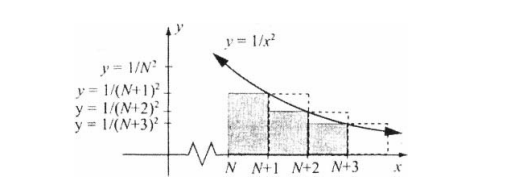
\includegraphics[max width=\textwidth]{fig52}
\caption{The areas of the shaded rectangles (that continue on indefinitely to the right) add up to precisely the Error $=\sum_{n=N+1}^{\infty} \frac{1}{n^{2}}$ of Example 5.6. But since they lie directly under the curve $y=1 / x^{2}$ from $x=N$ to $x=\infty$, we have Error $<$ Error Cap $\equiv \int_{N}^{\infty} \frac{d x}{x^{2}}$. }
\label{fig:fig_5_2}
\end{figure}

Let us now use MATLAB to perform this summation, following the principle of adding up the numbers in order of increasing size.

\begin{verbatim}
>> Sum=0; %initialize sum
>>for n=10000000:-1:1
Sum=Sum +1/n^2;
end
>> Sum ->Sum = 1.64493396684823 

\end{verbatim}

This took about 30 seconds on the author's PC. Since we know that the exact infinite sum is $\pi^{2} / 6$, we can look now at the actual error.

\begin{verbatim}
>> pi/s2/6-Sum
->ans = 9.999999495136080e-008 %This is indeed (just a wee bit) less than the desired
tolerance 10^-7. 
\end{verbatim}

 Let us look briefly at (6) (with $a_{n}=1 / n^{2}$ ) to see what kind of a bound on roundoff errors it gives for this computation. At each step, we are adding to the accumulated sum a quotient. Each of these quotients $\left(1 / n^{2}\right)$ gives a roundoff error (by (5)) at most $a_{n} u$. Combining this estimate with (6) gives the bound
 
$$
\begin{aligned}
&\left|\mathrm{fl}\left(S_{N}\right)-S_{N}\right| \leq 2 u\left\{\begin{array}{c}
{\left[\frac{9999999}{(10000000)^{2}}\right]+\left[\frac{9999999}{(9999999)^{2}}\right]+\left[\frac{9999998}{(9999998)^{2}}\right]+} \\
\cdots+\left[\frac{2}{(2)^{2}}\right]+\left[\frac{1}{(1)^{2}}\right]
\end{array}\right\}\\
&\leq 2 u\left\{\frac{1}{10000000}+\frac{1}{9999999}+\frac{1}{9999998}+\cdots+\frac{1}{2}+1\right\} \text {. }
\end{aligned}
$$

The sum in braces is $\sum_{n=1}^{10^{2}} \frac{1}{n}$. By a picture similar to the one of Figure 5.2, we can estimate this sum as follows: $\sum_{n=1}^{10^{7}} \frac{1}{n} \leq 1+\int_{1}^{N} \ln (x) d x=1+\ln (N)$. Since the unit roundoff for MATLAB is $2^{-53}$, we can conclude the following upper bound on the roundoff error of the preceding computation:
$$
\left|\mathrm{fl}\left(S_{N}\right)-S_{N}\right| \leq 2 u\left(1+\ln \left(10^{7}\right)\right) \approx 3.8 \times 10^{-15} \text {. }
$$
We thus have confirmation that roundoff error did not play a large role in this computation. Let's now see what happens if we perform the same summation in the opposite order.

\begin{verbatim}
» Sum=0;
» for n=1:10000000
Sum=Sum +1/n^2;
end
>> pi^2/6-Sum  ->ans = 1.000009668405966e-007
\end{verbatim}


Now the actual error is a bit worse than the desired tolerance of $10^{-7}$. The error estimate (6) would also be a lot larger if we reversed the order of summation. Actually for both of these floating point sums the roundoff errors were not very significant; such problems are called well-conditioned. The reason for this is that the numbers being added were getting small very fast. In the exercises and later in this book, we will encounter problems that are ill-conditioned, in that the roundoff errors can get quite large relative to the amount of arithmetic being done. The main difficulty in the last example was not roundoff error, but the computing time. If we instead wanted our accuracy to be $10^{-10}$, the corresponding calculation would take over 8 hours on the same computer! A careful look at the strategy we used, however, will allow us to modify it slightly to get a much more efficient method. A Better Approach: Referring again to Figure 5.2, we see that by sliding all of the shaded rectangles one unit to the right, the resulting set of rectangles will completely cover the region under the graph of $y=1 / x^{2}$ from $x=N+1$ to $x=\infty$. This gives the inequality:

$$
\text { Error } \left.>\int_{N+1}^{\infty} \frac{d x}{x^{2}}=\frac{x^{-1}}{-1}\right]_{x=N}^{x=\infty}=1 /(N+1) \text {. }
$$
In conjunction with the previous inequality, we have in summary that:
$$
\frac{1}{N+1}<\text { Error }<\frac{1}{N} \text {. }
$$
If we add to our approximation $S_{N}$ the average value of these two upper and lower bounds, we will obtain the following much better approximation for $S$ :
$$
\tilde{S}_{N} \equiv S_{N}+\frac{1}{2}\left[\frac{1}{N}+\frac{1}{N+1}\right] .
$$
The new error will be at most one-half the length of the interval from $1 /(N+1)$ to $1 / N$ :
$$
\left|S-\tilde{S}_{N}\right| \equiv \text { New Error } \leq \frac{1}{2}\left[\frac{1}{N}-\frac{1}{N+1}\right]=\frac{1}{2 N(N+1)}<\frac{1}{2 N^{2}} \text {. }
$$
(The elementary last inequality was written so as to make the new error bound easier to use, as we will now see.) With this new scheme much less work will be required to attain the same degree of accuracy. Indeed, if we wanted the error to be less than $10^{-7}$, this new scheme would require that the number of terms $N$ needed to sum should satisfy $1 / 2 N^{2} \leq 10^{-7}$ or $N \geq \sqrt{10^{7} / 2}=2236.07 \ldots$, a far cry less than the 10 million terms needed with the original method! By the same token, to get an error less than $10^{-10}$, we would need only take $N=70,711$ ! Let us now verify, on MATLAB, this 10-significant-digit approximation:

Now the actual error is a bit worse than the desired tolerance of $10^{-7}$. The error estimate (6) would also be a lot larger if we reversed the order of summation. Actually for both of these floating point sums the roundoff errors were not very significant; such problems are called well-conditioned. The reason for this is that the numbers being added were getting small very fast. In the exercises and later in this book, we will encounter problems that are ill-conditioned, in that the roundoff errors can get quite large relative to the amount of arithmetic being done. The main difficulty in the last example was not roundoff error, but the computing time. If we instead wanted our accuracy to be $10^{-10}$, the corresponding calculation would take over 8 hours on the same computer! A careful look at the strategy we used, however, will allow us to modify it slightly to get a much more efficient method.\\

\textbf{A Better Approach}: Referring again to Figure 5.2, we see that by sliding all of the shaded rectangles one unit to the right, the resulting set of rectangles will completely cover the region under the graph of $y=1 / x^{2}$ from $x=N+1$ to $x=\infty$. This gives the inequality

$$
\text { Error } \left.>\int_{N+1}^{\infty} \frac{d x}{x^{2}}=\frac{x^{-1}}{-1}\right]_{x=N}^{x=\infty}=1 /(N+1) \text {. }
$$
In conjunction with the previous inequality, we have in summary that:
$$
\frac{1}{N+1}<\text { Error }<\frac{1}{N} \text {. }
$$
If we add to our approximation $S_{N}$ the average value of these two upper and lower bounds, we will obtain the following much better approximation for $S$ :
$$
\tilde{S}_{N} \equiv S_{N}+\frac{1}{2}\left[\frac{1}{N}+\frac{1}{N+1}\right] .
$$
The new error will be at most one-half the length of the interval from $1 /(N+1)$ to $1 / N$ :
$$
\left|S-\tilde{S}_{N}\right| \equiv \text { New Error } \leq \frac{1}{2}\left[\frac{1}{N}-\frac{1}{N+1}\right]=\frac{1}{2 N(N+1)}<\frac{1}{2 N^{2}} \text {. }
$$
(The elementary last inequality was written so as to make the new error bound easier to use, as we will now see.) With this new scheme much less work will be required to attain the same degree of accuracy. Indeed, if we wanted the error to be less than $10^{-7}$, this new scheme would require that the number of terms $N$ needed to sum should satisfy $1 / 2 N^{2} \leq 10^{-7}$ or $N \geq \sqrt{10^{7} / 2}=2236.07 \ldots$, a far cry less than the 10 million terms needed with the original method! By the same token, to get an error less than $10^{-10}$, we would need only take $N=70,711$ ! Let us now verify, on MATLAB, this 10-significant-digit approximation:

\begin{verbatim}
» Sum=0; N=70711;
» for n=N:-l:l
Sum=Sum +1/n^2;
end
>> format long
>> Sum=Sum+(1/N +  1 / (N+1) ) /2          ->Sum = 1.64493406684823
>>abs(Sum-pi^2/6) ->ans =8.881784197001252e-016 
\end{verbatim}

The actual error here is even better than expected; our approximation is actually as good as machine precision! This is a good example where the (worst-case) error guarantee (New Error) is actually a lot larger than the true error. A careful examination of Figure $5.2$ once again should help to make this plausible.\\

We close this section with an exercise for the reader that deals with the approximation of an alternating series. This one is rather special in that it can be used to approximate the number $\pi$ and, in particular, we will be able to check the accuracy of our numerical calculations against the theory. We recall from calculus that an alternating series is an infinite series of the form $\sum(-1)^{n} a_{n}$, where $a_{n}>0$ for each $n$. Leibniz's Theorem states that if the $a_{n}$ 's decrease, $a_{n} \geq a_{n+1}$ for each $n$ (sufficiently large), and converge to zero, $a_{n} \rightarrow 0$ as $n \rightarrow \infty$, then the infinite series converges to a sum $S$. It furthermore states that if $S_{N}=\sum^{N}(-1)^{n} a_{n}$ denotes a partial sum (the lower index is left out since it can be any integer), then we have the error estimate: $\left|S-S_{N}\right| \leq a_{N+1}$.\\

EXERCISE FOR THE READER 5.5: Use the infinite series expansion:
$$
1-\frac{1}{3}+\frac{1}{5}-\frac{1}{7}+\cdots=\frac{\pi}{4} \text {, }
$$
to estimate $\pi$ with an error less than $10^{-7}$.\\

\hrule width \hsize \kern 1pt \hrule width \hsize height 0.4pt

\hspace{0.1cm}

\textbf{EXERCISES 5.3: }\\

NOTE: Unless otherwise specified, assume that all floating point arithmetic in these exercises is done in base 10.

\begin{enumerate}

\item (a) In chopped floating point arithmetic with $s$ digits and exponent range $m \leq e \leq M$, write down (in terms of these parameters $s, m$, and $M$ ) the largest positive floating point number and the smallest positive floating point number.

(b) Would these answers change if we were to use rounded arithmetic instead?

\item Recall that for two real numbers $x$ and $y$, the average value $(x+y) / 2$ of $x$ and $y$ lies between the values of $x$ and $y$.
 
(a) Working in a chopped floating point arithmetic system, find an example where $\mathrm{fl}((x+y) / 2)$ is strictly less than $\mathrm{nl}(x)$ and $\mathrm{f}(y)$.

(b) Repeat part (a) in rounded arithmetic.

\item (a) In chopped floating point arithmetic with base $\beta$, with $s$ digits and exponent range $m \leq e \leq M$, write down (in terms of these parameters $\beta, s, m$, and $M$ ) the largest positive floating point number and the smallest positive floating point number.

(b) Would these answers change if we were to use rounded arithmetic instead?

\item For each of the following arithmetic properties, either explain why the analog will be true in floating point arithmetic, or give an example where it fails. If possible, provide counterexamples that do not involve overflows, but take underflows to be zero.\\
(a) (\emph{Commutativity of Addition}) $x+y=y+x$\\
(b) (\emph{Commutativity of Multiplication}) $x \cdot y=y+x$\\
(c) (\emph{Associativity of Addition}) $x \cdot(y \cdot z)=(x \cdot y) \cdot z$\\
(d) (\emph{Distributive Law}) $x \cdot(y+z)=x \cdot y+x \cdot z$\\
(c) (\emph{Zero Divisors}) $x \cdot y=0 \Rightarrow x=0$ or $y=0$

\item Consider the infinite series: $1+\frac{1}{8}+\frac{1}{27}+\frac{1}{64}+\cdots \frac{1}{n^{3}}+\cdots$.\\
(a) Does it converge? If it does not, stop here; otherwise continue.\\
(b) How many terms would we have to sum to get an approximation to the infinite sum with an absolute ertor $<10^{-7}$ ?\\
(c) Obtain such an approximation.\\
(d) Using an approach similar to what was done after Example 5.6, add an extra term to the partial sums so as to obtain an improved approximation for the infinite series. How many terms would be required with this improved scheme? Perform this approximation and compare the answer with that obtained in part (c).

\item Consider the infinite series: $\sum_{n=1}^{\infty} \frac{1}{n \sqrt{n}}$.

(a) Does it converge? If it does not, stop here, otherwise continue.

(b) How many terms would we have to sum to get an approximation to the infinite sum with an absolute error $1 / 500$ ?

(c) Obtain such an approximation.

(d) Using an approach similar to what was done after Example $5.6$, add an extra term to the partial sums so as to obtain an improved approximation for the infinite series. How many terms would be required with this improved scheme? Perform this approximation and compare the answer with that obtained in part (c).

\item Consider the infinite series: $\sum_{n=1}^{\infty} \frac{(-1)^{n+1}}{n}=1-\frac{1}{2}+\frac{1}{3}-\frac{1}{4}+\cdots$.

(a) Show that this series satisfies the hypothesis of Leibniz's theorem (for $n$ sufficiently large) so that from the theorem, we know the series will converge to a sum $S$.

(b) Use Leibniz's theorem to find an integer $N$ so that summing up to the first $N$ terms only will give approximation to the sum with an error less than $.0001$.

(c) Obtain such an approximation.

\item Repeat all parts of Exercise 7 for the series: $\sum_{n=1}^{\infty}(-1)^{n} \frac{\ln n}{n}$.

\item (a) In an analogous fashion to what was done in Example 5.5, establish the following estimate for floating point multiplications of a set of $N$ positive real numbers, $P_{N}=a_{1} \cdot a_{2} \cdots a_{N}$ :

$$
\left|f\left(P_{N}\right)-P_{N}\right| \leq N u
$$
We have, as before, ignored higher-order error terms. Thus, as far as minimizing errors is concerned, unlike for addition, the roundoff errors do not depend substantially on the order of multiplication.

(b) In forming a product of positive real numbers, is there a good order to multiply so as to minimize the chance of encountering overflows or underflows? Explain your answer with some examples.

\item (a) Using an argument similar to that employed in Example 5.4, show that in base $\beta$ chopped floating point arithmetic the unit roundoff is given by $u=\beta^{1-3}$.
(b) Show that in rounded arithmetic, the unit roundoff is given by $u=\beta^{1-s} / 2$.

\item Compare and contrast a two-digit ( $s=2$ ) floating point number system in base $\beta=4$ and a fourdigit $(s=4)$ binary $(\beta=2)$ floating point number system.

\item In Exercise for the Reader 5.5, we used the following infinite series to approximate $\pi$ :

$$
\frac{\pi}{4}=1-\frac{1}{3}+\frac{1}{5}-\frac{1}{7} \cdots \Rightarrow \pi=4-\frac{4}{3}+\frac{4}{5}-\frac{4}{7} \cdots
$$
This altemating series was not a very efficient way to compute $\pi$, since it converges very slowly. Even to get an approximation with an accuracy of $10^{-7}$, we would need to sum about 20 million terms. In this problem we will give a much more efficient (faster-converging) series for computing $\pi$ by using Machin's identity $((13)$ of Chapter 2$)$ :
$$
\frac{\pi}{4}=4 \tan ^{-1}\left(\frac{1}{5}\right)-\tan ^{-1}\left(\frac{1}{239}\right)
$$
(a) Use this identity along with the arctangent's MacLaurin series (see equation (11) of Chapter 2) to express $\pi$ either as a difference of two alternating series, or as a single altemating series. Write your series both in explicit notation (as above) and in sigma notation.

(b) Perform an error analysis to see how many terms you would need to sum in the series (or difference of series) to get an approximation to $\pi$ with error $<10^{-7}$. Get MATLAB to perform this summation (in a "good" order) to thus obtain an approximation to $\pi$.

(c) How many terms would we need to sum so that the (exact mathematical) error would be less than $10^{-30}$ ? Of course, MATLAB only uses 16-digit floating point arithmetic so we could not directly use it to get such an approximation to $\pi$ (Unless we used the symbolic toolbox; see Appendix A).

\item Here is $\pi$, accurate to 30 decimal places:

$$
\pi=3.141592653589793238462643383279 \ldots
$$
Can you figure out a way to get MATLAB to compute $\pi$ to 30 decimals of accuracy without using its symbolic capabilities?

\textbf{Suggestions}: What is required here is to build some MATLAB functions that will perform certain mathematical operations with more significant digits (over 30) than what MATLAB usually guarantees (about 15). In order to use the series of Exercise 12, you will need to build functions that will add/subtract, and multiply and divide (at least). Here is an example of a possible syntax for such new function: $z=$ highaccuracyadd $(x, y)$ where $x$ and $y$ are vectors containing the mantissa (with over 30 digits) as well as the exponent and sign (can be stored as 1 for plus, 2 for negative in one of the slots). The output $z$ will be another vector of the same size that represents a $30+$-significant-digit approximation to the sum $x+y$. This is actually quite a difficult problem, but it is fun to try.


\end{enumerate}

\end{document}